\section{Intraprocedural Profiling}

{\em Path profiling} is a powerful {\em intraprocedural} methodology for identifying performance bottlenecks in a program, and has received considerable attention in the last 15 years for its practical relevance. The well-known Ball and Larus numbering algorithm~\cite{Ball96} can efficiently encode {\em acyclic} paths that are taken across the control-flow graph of a function. Previous attempts to extend it to {\em cyclic} paths, as spanning multiple loop iterations, to capture more optimization opportunities, are based on rather complex algorithms that incur severe performance overheads even for short cyclic paths. In this thesis we present a new, data-structure based approach to {\em multi-iteration} path profiling built on top of the original Ball-Larus numbering technique. Starting from the observation that a cyclic path can be described as a concatenation of Ball-Larus acyclic paths, we show how to accurately profile all executed paths obtained as a concatenation of up to $k$ Ball-Larus paths, where $k$ is a user-defined parameter.

%{\em Path profiling} is a powerful {\em intraprocedural} methodology for identifying performance bottlenecks in a program, and has received considerable attention in the last 15 years for its practical relevance. The well-known Ball and Larus algorithm~\cite{Ball96} for {\em intraprocedural} path profiling can efficiently encode {\em acyclic} paths that are taken across the control-flow graph of a function. Previous attempts to extend it to encode {\em cyclic} paths, and thus to span multiple loop iterations in order to capture more optimization opportunities, are based on rather complex algorithms that incur severe performance overheads even for short cyclic paths. In this thesis we present a new, data-structure based approach to {\em multi-iteration} path profiling built on top of the original Ball-Larus numbering technique. Starting from the observation that any cyclic path can be described as a concatenation of Ball-Larus acyclic paths, we show how to accurately profile all executed paths obtained as a concatenation of up to $k$ Ball-Larus paths, where $k$ is a user-defined parameter.

%We provide examples showing that this method can reveal optimization opportunities that acyclic-path profiling would miss, and we present an extensive experimental investigation on a large variety of Java benchmarks in the Jikes RVM. Experiments show that our approach can be even faster than a hash table-based implementation of the Ball-Larus algorithm due to fewer operations on smaller tables, producing compact representations of cyclic paths even for large values of $k$.

\subsection{Motivation and Contributions}

Path profiling associates performance metrics, usually frequency counters, to paths taken in the control flow graph of a routine. Identifying the hottest paths can direct optimizations to portions of the code where most resources are consumed, often yielding significant speedups. For instance, trace scheduling can improve performance by increasing instruction-level parallelism along frequently executed paths~\cite{Fisher81,Young98}. Although basic block and edge profiles are inexpensive and widely available, they do not always correctly predict frequencies of overlapping paths. 

The seminal paper by Ball and Larus~\cite{Ball96} introduced a simple and elegant path profiling technique. The main idea was to implicitly number all possible acyclic paths in the control flow graph so that each path is associated with a unique compact path identifier (ID). The authors showed that path IDs can be efficiently generated at runtime and can be used to update a table of frequency counters. Although in general the number of acyclic paths may grow exponentially with the graph size, in typical control flow graphs this number is usually small enough to fit in current machine word-sizes, making this approach very effective in practice.

While the original Ball-Larus approach was restricted to acyclic paths obtained by cutting paths at loop back edges, profiling paths that span consecutive loop iterations is a desirable, yet difficult, task that can yield better optimization opportunities. Consider, for instance, the problem of eliminating redundant executions of instructions, such as loads and stores~\cite{Bodik99}, conditional jumps~\cite{Bodik97}, expressions~\cite{Bodik98,Bodik04}, and array bounds checks~\cite{Bodik00}. A typical situation is that the same instruction is redundantly executed at each loop iteration, which is particularly common for arithmetic expressions and load operations~\cite{Bodik04,Bodik99}. To identify such redundancies, paths that extend across loop back edges need to be profiled. Another application is trace scheduling~\cite{Young98}: if a frequently executed cyclic path is found, compilers may unroll the loop and perform trace scheduling on the unrolled portion of code. Tallam {\em et al.}~\cite{Tallam04} provide a comprehensive discussion of the benefits of multi-iteration path profiling.

Different authors have proposed techniques to profile cyclic paths by modifying the original Ball-Larus path numbering scheme in order to identify paths that extend across multiple loop iterations~\cite{Tallam04,Roy09,Li12}. Unfortunately, all known solutions require rather complex algorithms that incur severe performance overheads even for short cyclic paths, leaving the interesting open question of finding simpler and more efficient alternative methods.

\paragraph*{Contributions.} In this thesis, we present a novel, data structure-based approach to multi-iteration path profiling. Our method stems from the observation that any cyclic execution path in the control flow graph of a routine can be described as a concatenation of Ball-Larus acyclic paths (BL paths). In particular, we show how to accurately profile {\em all executed paths} obtained as a concatenation of up to $k$ BL paths, where $k$ is a user-defined parameter. We reduce multi-iteration path profiling to the problem of counting $n$-grams, i.e., contiguous sequences of $n$ items from a given sequence. To compactly represent collected profiles, we organize them in a forest of prefix trees (or tries)~\cite{Fredkin60} of depth up to $k$, where each node is labeled with a BL path, and paths in a tree represent concatenations of BL paths that were actually executed by the program, along with their frequencies. We also present an efficient construction algorithm based on a variant of the \ksf\ data structure presented in~\cite{Ausiello12}. 

\subsection{Approach}

Differently from previous techniques~\cite{Tallam04,Roy09,Li12}, which rely on modifying the Ball-Larus path numbering to cope with cycles, our method does not	require
\ifdefined\noauthorea
\begin{wrapfigure}{l}{0.5\textwidth}
\vspace{-2mm}
\centering
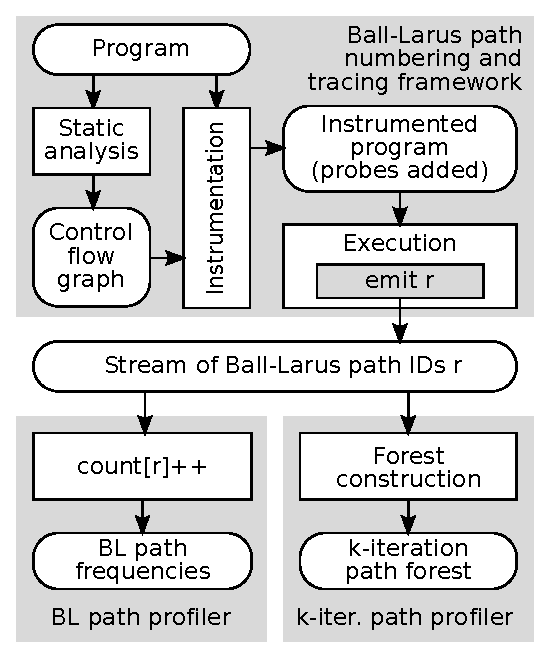
\includegraphics[width=0.45\textwidth]{figures/kblpp-approach/kblpp-approach.eps}
\caption{\protect\label{fig:kblpp-approach} Overview of our approach: Ball-Larus profiling versus k-iteration path profiling, cast in a common framework.
%Overview of our approach: classical Ball-Larus profiling versus k-iteration path profiling, cast in a common framework.
}
\end{wrapfigure}
%\vspace{2mm}
\noindent
\fi
any modification of the original numbering technique described in~\cite{Ball96}. The main idea behind our approach is to fully decouple the task of tracing Ball-Larus acyclic paths at run time from the task of concatenating and storing them in a data structure to keep track of multiple iterations. The decoupling is performed by letting the Ball-Larus profiling algorithm issue a stream of BL path IDs (see \myfigure\ref{fig:kblpp-approach}), where each ID is generated when a back edge in the control flow graph is traversed or the current procedure is abandoned. As a consequence of this modular approach, our method can be implemented on top of existing Ball-Larus path profilers, making it simpler to code and maintain.

%~\cite{}

\subsection{Algorithms}

\subsection{Discussion}

\subsection{Comparison with Related Work}